\chapter{Planificación}

En la tabla~\ref{tab:plan} se puede observar la planificación del proyecto.

\begin{table}[h]
	\centering
	\caption{Planificación del proyecto.}\label{tab:plan}
	\begin{tabular}{ccccc}
		\toprule
		\textbf{Tarea} & \emph{Dependencias} & \emph{Recurso} & \emph{Días} & \emph{Horas} \\
		\midrule
		T1	&				& Jefe de proyecto			& 1		&	4	\\
		T2	&				& Jefe de proyecto			& 1		&	4	\\
		T3	&	T1			& Programador				& 8		&	32	\\
		T4	&	T2			& Diseñador					& 4		&	16	\\
		T5	&	T3			& Programador				& 14	&	56	\\
		T6	&	T4			& Diseñador					& 7		&	28	\\
		T7	&	T5, T6		& Experto en WebLab-Deusto	& 8		&	32	\\
		T8	&	T7			& Jefe de proyecto			& 1		&	2	\\
		T9	&	T8			& Programador				& 2		&	8	\\
		T10	&	T9			& Programador				& 8		&	32	\\
		T11	&	T10			& Experto en WebLab-Deusto	& 4		&	16	\\
		T12	&	T11			& Jefe de proyecto			& 2		&	8	\\
		T13	&	T12			& Programador				& 5		&	20	\\
		T14	&	T13			& Programador				& 5		&	20	\\
		T15	&	T12			& Diseñador					& 4		&	16	\\
		T16	&	T14, T15	& Experto en WebLab-Deusto	& 12	&	48	\\
		T17	&	T7			& Jefe de proyecto			& 3		&	12	\\
		\bottomrule
	\end{tabular}
\end{table}

Podemos además ver el diagrama de Gantt en la figura~\ref{fig:gantt}. También tenemos el diagrama de precedencias en la figura~\ref{fig:web}.

\begin{figure}
	\centering
	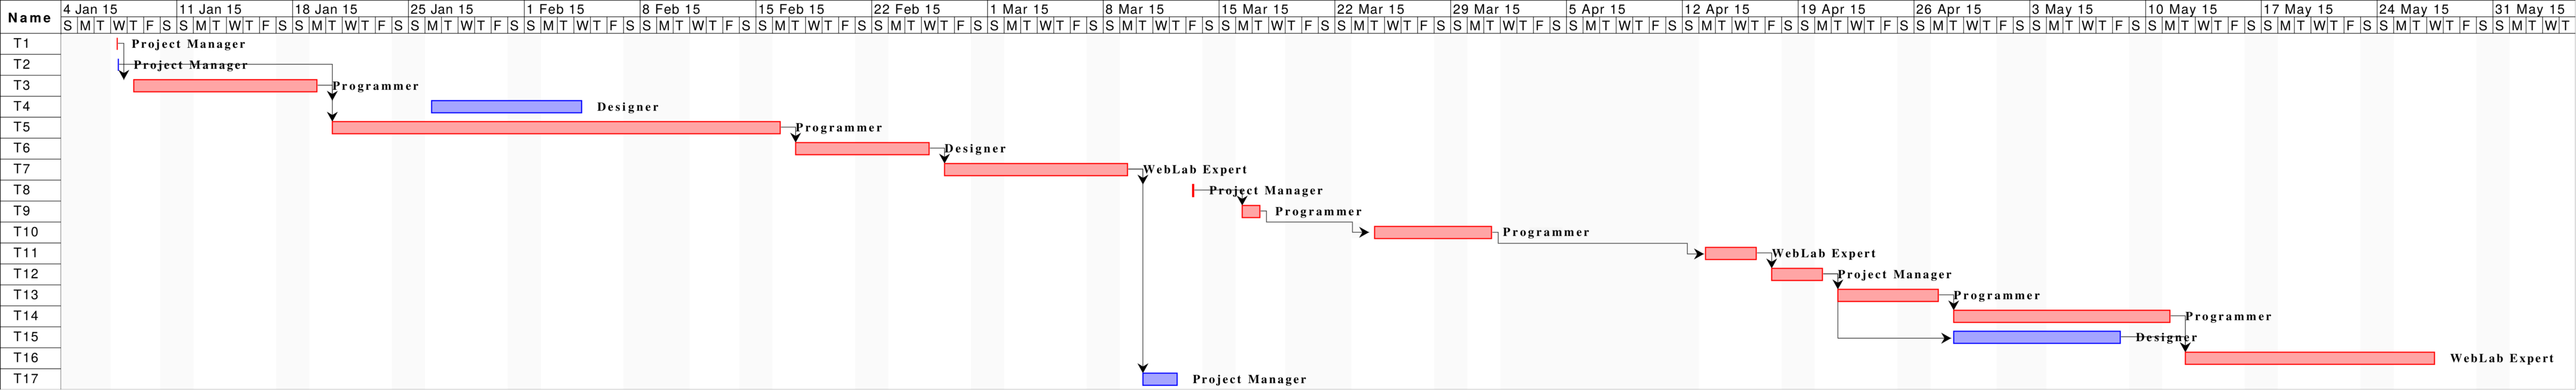
\includegraphics[width=\textheight, angle=-90]{fig/gantt}
	\caption{Diagrama de Gantt del proyecto.}\label{fig:gantt}
\end{figure}

\begin{figure}
	\centering
	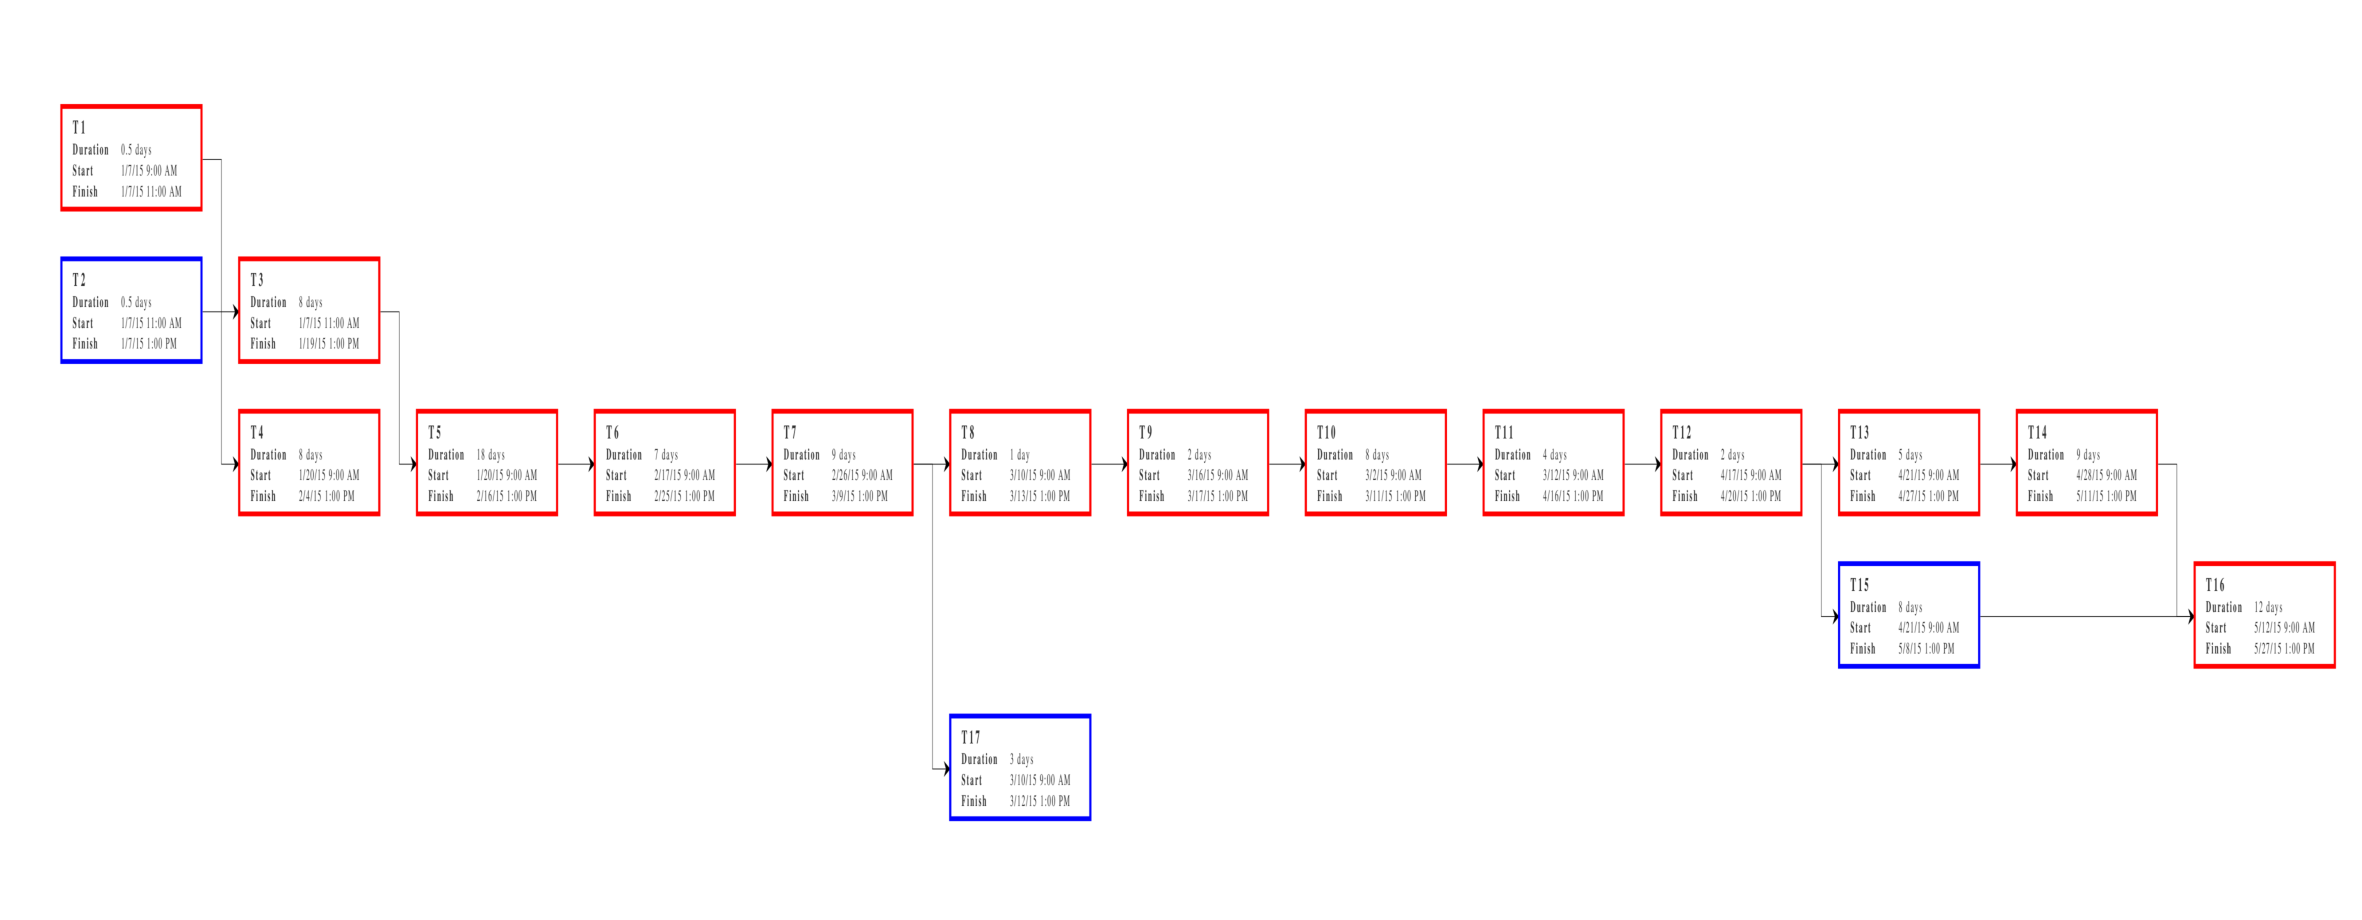
\includegraphics[width=\textheight, angle=-90]{fig/web}
	\caption{Diagrama de red del proyecto.}\label{fig:web}
\end{figure}
